\chapter{এক্সচেঞ্জ আর্গুমেন্ট}

\section{প্রমাণ দাও}

সাধারণত গ্রিডি অ্যালগরিদম গুলো অনেকটা এরকম হয়ঃ যতক্ষণ পর্যন্ত সম্ভব প্রদত্ত শর্তগুলো ঠিক রেখে তুমি প্রতিবার একটি করে ইলিমেন্ট সিলেক্ট করে তোমার সলিউশনে অ্যাড করবা যেটায় তোমার সবচেয়ে বেশি লাভ হয়। আমরা এক্সচেঞ্জ আর্গুমেন্ট ব্যবহার করে যেমন আমাদের এই গ্রিডি অ্যালগরিদমের শুদ্ধতা প্রমাণ করতে পারি, তেমনি এক্সচেঞ্জ আর্গুমেন্ট এর ধাপ গুলো নিয়ে চিন্তা করতে গিয়ে আমাদের গ্রিডি সলিউশনও দাঁড় করিয়ে ফেলতে পারবো অনেক সময়। এক্সচেঞ্জ আর্গুমেন্ট প্রুফ গুলোর মেইন আইডিয়া হলো, তুমি যেকোনো একটি অপ্টিমাল সলিউশন নিবে, তারপর সেটিকে ধাপে ধাপে এমনভাবে তোমার গ্রিডি সলিউশনে পরিবর্তন করবে যেন প্রতি ধাপে তোমার কোন লস না হয়। তাহলে তুমি বলতে পারবে অন্তত এমন একটা অপ্টিমাল সলিউশন আছে, যেটা কিনা তোমার গ্রিডি সলিউশনের চাইতে খারাপ অথবা একই। অন্যভাবে বলতে গেলে, তোমার সলিউশনও একটি অপ্টিমাল সলিউশন। একটা উদাহরণ দেখা যাক।

\begin{example}[ডট প্রডাক্ট মিনিমাইজেশন]
তোমাকে দুটি অ্যারে দেওয়া আছে। তোমাকে এমনভাবে অ্যারে দুটিকে রিঅ্যারেঞ্জ করতে হবে যেন তাদের ডট গুণফল অর্থাৎ, $\sum_{i=1}^{N} A_i B_i$ এর মান মিনিমাম হয়।
\end{example}
\begin{solution}
আমরা চাই না দুটি বড় বড় সংখ্যা একসাথে থাকুক কারণ তাদের গুণফল অবশ্যই বড় হয়ে যাবে। অন্যদিকে, দুটি ছোট ছোট সংখ্যা একসাথে থাকলে লাভ হতে পারে বলে মনে হতে পারে। কিন্তু এরকম করলে বড় বড় সংখ্যা গুলো একসাথে হয়ে যাবে। তাহলে এরকম একটা কিছু করা যায়- একটি ছোট আর একটি বড় সংখ্যা একসাথে পেয়ারআপ করা। এই আইডিয়াটাকে গুছিয়ে বললে হবে- প্রথম অ্যারেটিকে নন-ডিক্রিজিং অর্ডারে সর্ট করা এবং দ্বিতীয় অ্যারেটিকে নন-ইনক্রিজিং অর্ডারে সর্ট করা। এখন আমাদের প্রমাণ করতে হবে, এটি একটি অপ্টিমাল সলিউশন। আমরা ধরে নিতে পারি প্রথম অ্যারেটি নন-ডিক্রিজিং অর্ডারে সর্ট করা আছে। এখন ধরো এমন একটা অপ্টিমাল সলিউশন আছে যেখানে $B$ ডিক্রিজিং অর্ডারে সর্ট করা নেই, অর্থাৎ, এমন একটা $i$ আছে যেন, $B_{i} < B_{i+1}$।  এখন আমরা এদেরকে সোয়াপ করে আমাদের গ্রিডি সলিউশনের দিকে যেতে চাই। যদি সোয়াপ করি, তাহলে আমদের গুণফলে যেই অতিরিক্ত কস্ট অ্যাড হবে তা হলোঃ $A_iB_{i+1} + A_{i+1}B_i - A_iB_i - A_{i+1}B_{i+1}$।  সুতরাং আমাদের প্রমাণ করতে হবে-
\begin{align*}
	A_iB_{i+1} + A_{i+1}B_i - A_iB_i - A_{i+1}B_{i+1} &\le 0 & \\
	A_i(B_{i+1} - B_i) - A_{i+1}(B_{i+1} - B_i) &\le 0\\
	A_i &\le A_{i+1} &\text{কারণ, $B_{i+1} - B_i > 0$}
\end{align*}
আসলেই তাই! (ইমপ্লিকেশন গুলো উল্টা অর্ডারে লিখতে হবে আরকি ফর্মাল প্রুফে...) তাহলে আমরা প্রুফ করে ফেললাম- এভাবে সোয়াপ করতে থাকলে আমরা কোন লস ছাড়াই অপ্টিমাল সলিউশন থেকে গ্রিডি সলিউশনে পৌছাতে পারবো (খেয়াল করো, শুধুমাত্র দুটো পাশাপাশি উপাদান সোয়াপ করে করেই কিন্তু একটি সিকুয়েন্সের যেকোনো পারমুটেশনে পৌছনো যায়)। অর্থাৎ, আমাদের গ্রিডি সলিউশনও একটি অপ্টিমাল সলিউশন!
\end{solution}

\section{মুল টেকনিক}

গ্রিডি অ্যালগরিদম বের করার পরে তা এক্সচেঞ্জ আর্গুমেন্ট দিয়ে প্রমাণ করার জন্য আমরা যা করি তাকে মূলত নিচের ৩টা স্টেপে ভাগ করা যায়-
\begin{enumerate}
	\item ধরলাম আমাদের গ্রিডি অ্যালগরিদম ব্যবহার করে আমরা একটা সলিউশন $G = \cbra{g_1, g_2, \ldots, g_n}$ পেয়েছি, আর $O = \cbra{o_1, o_2, \ldots, o_m}$ একটি অপ্টিমাল সলিউশন।  এখানে কিন্তু আমরা ধরে নিচ্ছি $G$ আর $O$ দুটোই সবরকমের শর্ত মেনেই বানানো হয়েছে।
	\item ধরে নাও $G \not= O$ আর  তাদের মধ্যে পার্থক্য করো, যেমন, ধর $G$ তে এমন একটি উপাদান পেলে যেটি $O$ তে নেই (অথবা, $O$ তে এমন একটি উপাদান পেলে যেটি $G$ তে নেই) অথবা এমন দুটি উপাদান আছে যারা $G$ তে যেই অর্ডারে আছে, $O$ তে তার বিপরীত অর্ডারে আছে।
	\item \textbf{এক্সচেঞ্জ।} যেমন, প্রথম কেইস এর জন্য $O$ থেকে একটি উপাদান বের করে আরেকটি উপাদান ঢুকালা, অথবা দ্বিতীয় কেইস এর জন্য অর্ডারটা সোয়াপ করে দিলে (বেশিরভাগ সময় খালি পাশাপাশি ২টা উপাদান নিয়েই কাজ করা হয়)। এখন কারণ দেখাও, এক্সচেঞ্জ করার পর তোমার নতুন সলিউশনটা আগেরটার তুলোনায় খারাপ না এবং এরপর দেখাবে তুমি যদি এইরকম এক্সচেঞ্জ করতে থাকো তাহলে একসময় $O$ কে $G$ এর সমান বানাতে পারবে। সুতরাং তোমার গ্রিডি সলিউশন যেকোনো অপ্টিমাল সলিউশনের (বা যেকোনো নন-অপ্টিমাল সলিউশনের) চাইতে ভাল বা সমান, যার মানে দাঁড়ালো তোমার সলিউশনও একটি অপ্টিমাল সলিউশন।
\end{enumerate}

অনেক ভারী ভারী আলোচনা হয়ে গেলো! আসলে প্রথমেই যে বলেছিলাম এক্সচেঞ্জ আর্গুমেন্ট দিয়ে প্রুফ করতে গিয়ে আমরা অনেকসময় গ্রিডি সলিউশনও দাঁড় করিয়ে ফেলতে পারি- এভাবে চিন্তা করলে আমরা কিছু কন্ডিশন পাই (যেমন পাশাপাশি ২টা উপাদানের মধ্যে কিরকম সম্পর্ক হতে পারে) এবং সেগুলো থেকে আমরা উপাদান গুলোর একটি অর্ডারিং পেতে পারি যেটা আমাদের কাজকে অনেক সহজ করে দেয়। আশা করি পরের অংশের উদাহরণগুলো দেখলে বিষয়টা পরিষ্কার হবে।

\begin{exercise}
দুটি অ্যারে দেওয়া আছে (একই উপাদান বার বার থাকতে পারে)। অ্যারে দুটির উপাদানের মাল্টিসেট গুলো সমান, অর্থাৎ, এদেরকে সর্ট করলে অ্যারে দুটি একই হবে। তুমি প্রতি ধাপে প্রথম অ্যারেটির দুটি পাশাপাশি উপাদান সোয়াপ করতে পারবা। মিনিমাম কয়টি মুভে প্রথম অ্যারেটিকে তুমি দ্বিতীয় অ্যারের সমান করতে পারবে তা বের করতে হবে।
\end{exercise}

\section{ডিপির সাথে সম্পর্ক}

আমরা যখন কিছু উপাদানের উপর ডিপি করি তখন আমরা কোন কোন উপাদানগুলো বিবেচনা করে ফেলেছি এবং কোনগুলো বাকি আছে তার হিসাব রাখতে হয় এবং বেশিরভাগ ক্ষেত্রেই তা একটি প্রিফিক্স বা সাফিক্স হয়। অর্থাৎ আমাদের $\mathcal{O}(N)$ সাইজের একটা স্টেট রাখতে হয়। কিন্তু মনে করো আমাদের এরকম কিছু করতে বলল-
\begin{enumerate}
  \item উপাদানগুলোর একটি অপ্টিমাল সাবসেট বাছাই করতে হবে।
  \item এরপর চেক করে দেখতে হবে, ঐ সাবসেটটিকে কি এমন কোনো অর্ডারে সাজানো যায় কিনা যাতে সেই অর্ডারিং প্রবলেমে দেওয়া কিছু শর্ত পালন করে।
  \item যদি করে, তাহলে সেই সাবসেটটিকে আমরা গ্রহণযোগ্য ধরব।
  \item আবার একটি গ্রহণযোগ্য সাবসেটের উপাদান গুলো কিভাবে সাজানো আছে, তার উপর প্রবলেমে দেওয়া কস্ট ফাংশান ডিপেন্ড করে। সুতরাং, একটি সাবসেট বাছাই করে, তার মধ্যে আবার উপাদান গুলো এমন ভাবে সাজাতে হবে যেন কস্ট ফাংশান মিনিমাইজ হয়।
  \item সব গ্রহণযোগ্য সাবসেটের মধ্যে মিনিমাম কস্ট বের করতে হবে।
\end{enumerate}
তখন কি করা যায়? এমন প্রবলেম দেখলে মনে হতে পারে কোন গ্রিডি সলিউশন বের করতে পারি কিনা দেখি। হয়তো তুমি পেয়েও যেতে পারো! কিন্তু এরকম সমস্যায় এক্সচেঞ্জ আর্গুমেন্ট এর টেকনিকটিও অ্যাপ্লাই করে দেখা উচিত। এক্সচেঞ্জ আর্গুমেন্ট অ্যাপ্লাই করে আমরা উপাদানগুলোর একটি অর্ডার পেতে পারি যেখানে অন্তত একটি অপ্টিমাল আন্সারে উপাদানগুলো সেই অর্ডার অনুযায়ী সাজানো থাকবে। এতে যেই সুবিধা হয় তা হলো, এরপর আমরা প্রিফিক্সের/সাফিক্সের উপর ডিপি করতে পারবো।

\begin{example}[\href{https://atcoder.jp/contests/cf17-final/tasks/cf17\_final\_d}{Code Festival '17 Final D - Zabuton}]
\label{pillow_tower}
একটি বালিশ প্রতিযোগিতায় $N \le 5\times 10^3$ জন প্রতিযোগী আছে। প্রত্যেক প্রতিযোগীর জন্য ২টি সংখ্যা- তার উচ্চতা $(0 \le h_i \le 10^9)$ এবং তার কাছে কয়টি বালিশ আছে ($1 \le p_i \le 10^9$) তা তোমাকে দেওয়া আছে। প্রতিযোগীদের নির্দিষ্ট একটি ক্রমে সাজানোর পর তারা সেই ক্রমে একে একে আসে এবং স্তূপে বালিশের সংখ্যা দেখে (প্রথমে ০ থাকবে)। যদি স্তূপে তার নিজের \textbf{উচ্চতার} চেয়ে \textbf{বেশি} সংখ্যক বালিশ থাকে তাহলে সে মন খারাপ করে চলে যায়, নতুবা তার কাছে যতটি বালিশ আছে সেগুলো সে স্তূপে রেখে দেয়। তোমাকে বের করতে হবে কিভাবে প্রতিযোগীদের সাজালে সর্বোচ্চ সংখ্যক প্রতিযোগী বালিশ রাখতে পারবে (মন খারাপ করবে না)। তোমাকে শুধু সেই সর্বোচ্চ সংখ্যাটি আউটপুট দিতে হবে।
\end{example}
\begin{solution}
মনে করো এমন একটি সাজানোর উপায় আছে যাতে সবাই বালিশ রাখতে পারে (আসলে তো না-ই থাকতে পারে, কিন্তু আমরা প্রথমে সিম্পল জিনিস নিয়ে ঘাঁটাঘাঁটি করে দেখি না কি পাই)। ধরো, $O$ হলো এমন একটি সাজানোর উপায়। আমরা এক্সচেঞ্জ আর্গুমেন্ট অ্যাপ্লাই করে বের করার চেষ্টা করবো এদের মধ্যে সম্পর্ক কেমন হতে পারে। $O$ এর কিছু প্রপার্টি লিখে শুরু করা যাক।
$O$ তে পাশাপাশি আছে এমন ২টি প্রতিযোগী নাও আর ধরো $P$ হলো $i$ এর আগে আসা প্রতিযোগীদের বালিশের সংখ্যার যোগফল, অর্থাৎ, $P = \sum_{j=1}^{i-1} p_i$। এখন, $O$ একটি ভ্যালিড অর্ডারিং হবে যদি এবং কেবল যদিঃ
\begin{align}
  P & \le h_i \text{ এবং} \label{pillow:eq1} \\
  P + p_i & \le h_{i+1} \label{pillow:eq2}
\end{align}
হতে হবে। এখন নিচের দুটির মধ্যে যেকোনো একটি হতে পারেঃ
\begin{enumerate}
  \item \textbf{$i$ এবং  $i+1$ এক্সচেঞ্জ করা যাবে না।} অর্থাৎ, $i$ তম এবং $i+1$ তম প্রতিযোগীর অবস্থান যদি আমরা পরিবর্তন করে দেই তাহলে $O$ একটি ভ্যালিড সিকুয়েন্স থাকবে না। অন্যভাবে বলতে গেলে-
  \begin{align}
    h_{i+1} & < P \text{ \textbf{অথবা}} \label{pillow:eq3} \\
    h_i & < P + p_{i+1} \label{pillow:eq4}
  \end{align}
  হতে হবে। খেয়াল করো, \eqref{pillow:eq2} সত্য হলে \eqref{pillow:eq3} সত্য হতে পারে না। সুতরাং, \eqref{pillow:eq4}-কে সত্য হতে হবে। \eqref{pillow:eq1}, \eqref{pillow:eq2} এবং \eqref{pillow:eq4} থেকে হিসাব করে পাই-
  \begin{align}
    p_i + h_i &< p_{i+1} + h_{i+1} \label{pillow:eq5}
  \end{align}
  -একটি কমপ্লিট অর্ডার! কিন্তু এর মানে কি আসলে? \eqref{pillow:eq5} আমাদের বলছে, অপ্টিমাল সিকুয়েন্সের পাশাপাশি দুটি উপাদান যদি এক্সচেঞ্জ করা না যায় তাহলে তারা \eqref{pillow:eq5} শর্ত পূরণ করে। কিন্তু আমাদের তো আরেকটি কেইস বাকি রয়ে গিয়েছে! তখন কি হবে?
  \item \textbf{$i$ এবং $i+1$ এক্সচেঞ্জ করা যাবে।} তাহলে,
  \begin{align}
    P &\le h_{i+1} \text{ এবং} \label{pillow:eq6} \\
    P + p_{i+1} &\le h_i \label{pillow:eq7}
  \end{align}
  হতে হবে। একটু খেয়াল করলে দেখবে \eqref{pillow:eq7} $\implies$ \eqref{pillow:eq1} এবং \eqref{pillow:eq2} $\implies$ \eqref{pillow:eq6}। তাই \eqref{pillow:eq1} আর \eqref{pillow:eq6} আমাদের চিন্তা থেকে বাদ দিয়ে দিতে পারি। আরেকটা খুবই সুন্দর জিনিস হলো, \eqref{pillow:eq5} এবং \eqref{pillow:eq7} থেকে আমরা বলতে পারি \eqref{pillow:eq2} সত্য হবে। আবার আমরা আগেই দেখেছি \eqref{pillow:eq7} সত্য হলে \eqref{pillow:eq1} সত্য হবে। অর্থাৎ, আমরা যদি এক্সচেঞ্জ করতে পারি, তাহলে \eqref{pillow:eq5} অনুযায়ী সাজালেও $O$ একটি ভ্যালিড সিকুয়েন্স থাকবে!
\end{enumerate}

মোটকথা হলো, যদি অন্তত একটি ভ্যালিড অ্যারেঞ্জমেন্ট থাকে তাহলে প্রতিযোগীদের \eqref{pillow:eq5} অনুযায়ী সর্ট করলে সেটিও একটি ভ্যালিড সিকুয়েন্স হবে! এখন তাহলে আমাদের কাজ হলো ইনপুটে দেওয়া প্রতিযোগীদের \eqref{pillow:eq5} দিয়ে সর্ট করার পর \eqref{pillow:eq1} এবং \eqref{pillow:eq2} শর্ত পালন করে এমন ম্যাক্সিমাম লেংথের সাবসিকুয়েন্স বের করা। এই কাজটি আমরা একটি সাধারণ ডিপি দিয়েই করতে পারি।

$dp_{i,P}$ এর মান হলো- প্রথম $i$ টি উপাদান বিবেচনা করলে ম্যাক্সিমাম ভ্যালিড সাবসিকুয়েন্সের লেংথ যাতে সাবসিকুয়েন্সের $p_i$ গুলোর যোগফল $P$ এর সমান হয়। এটার ট্রানজিশন অনেক সোজা। কিন্তু আসল কথা হলো, $P$ এর মান তো অনেক বড় হতে পারে!

\textbf{ডিপির স্টেট এবং ভ্যালু সোয়াপ করা।} আমরা আগেই ডিপির স্টেট-ভ্যালু সোয়াপ করার কিছু উদাহরণ দেখে এসেছি। এখানেও আমাদের সেটি লাগবে। আমাদের নতুন ডিপি $dp_{i,j}$ এর মান হলো কোন একটি $j$ সাইজের ভ্যালিড সাবসিকুয়েন্সের মিনিমাম $\sum p_i$ এর মান। এটার ট্রানজিশনও সোজা, পাঠকের অনুশীলনীর জন্য আর বলে দেওয়া হচ্ছে  না।
\end{solution}

\begin{example}[\href{https://oj.uz/example/view/JOI19\_lamps}{JOI Spring Camp '19 - Lamps}]
তোমাকে দুটি $N$ সাইজের বাইনারি অ্যারে $A$ আর $B$ দেওয়া আছে। তুমি প্রতি ধাপে নিচের যেকোনো একটি অপারেশন $A$ অ্যারের উপর প্রয়োগ করতে পারবা-
\begin{enumerate}
	\item \textbf{সেট অপারেশনঃ} একটি রেঞ্জ $[l, r]$ যেখানে $1 \le l \le r \le N$ বাছাই করে $A[l \ldots r]$ এর সব মান $0$ করে দিবে।
	\item \textbf{রিসেট অপারেশনঃ} একটি রেঞ্জ $[l, r]$ যেখানে $1 \le l \le r \le N$ বাছাই করে $A[l \ldots r]$ এর সব মান $1$ করে দিবে।
	\item \textbf{টগল অপারেশনঃ} একটি রেঞ্জ $[l, r]$ যেখানে $1 \le l \le r \le N$ বাছাই করে $A[l \ldots r]$ এর সব মান পরিবর্তন করে দিবে (০ থাকলে ১ আর ১ থাকলে ০ করতে হবে)।
\end{enumerate}
তোমাকে বের করতে হবে মিনিমাম কয়টি অপারেশনে তুমি $A$ অ্যারেকে $B$ এর সমান করতে পারবে।
\end{example}
\begin{solution}
যদিও বেশিরভাগ অপটিমাইজেশন প্রবলেমই হয় গ্রিডি না হয় ডিপি হয়, তাও কেও যদি এইধরনের প্রবলেম আগে কখনো না দেখে থাকে তাহলে এটা যে আদৌ ডিপি প্রবলেম, তা আন্দাজ করারও উপায় আছে বলে আমি মনে করি না। প্রবলেমটা সম্পর্কে কিছু আইডিয়া পাওয়ার জন্য আমরা একটি মিনিমাম অপারেশনের সিকুয়েন্স কেমন হতে পারে তা চিন্তা করতে পারি। ধরো এমন একটা সিকুয়েন্স হলো $o_1, o_2, \ldots, o_k$ (তাহলে $k$ হলো আমাদের উত্তর, আর, একটা অপারেশনকে আমরা একটা টুপল $o_i = (l_i, r_i, \star_i)$ দিয়ে বর্ণনা করবো)।  এখন আমরা একটু খতিয়ে দেখবো, একটা অপারেশন আরেকটা অপারেশনের ওপর কিভাবে প্রভাব ফেলছে। দুটো অপারেশন $o_i$ আর $o_j$ নাও ($i < j$)। এখন দেখো, যদি $j > i+1$ হয় তাহলে ঐ দুটি অপারেশনের মাঝে আরও অনেক অপারেশন এসে আমাদের ঝামেলায় ফেলে দিচ্ছে। তাই আমরা আপাতত $j=i+1$ ধরি, অর্থাৎ $o_i$ আর $o_{i+1}$ নিয়ে চিন্তা করবো আমরা এখন। আমরা এবার এই অপারেশন দুটো কোনোভাবে কম্বাইন করে একটি অপারেশন বানানোর চেষ্টা করবো যাতে আমাদের অপারেশনের সংখ্যা কমে যায়। কিন্তু আমরা তো একটা মিনিমাম সাইজের সিকুয়েন্স নিয়েছিলাম! হ্যাঁ, আমরা যদি ঐ ২টা অপারেশন কম্বাইন করতে পারি, তাহলে এমন বৈশিষ্ট্যের ২টি অপারেশন আমরা কোন অপ্টিমাল সিকুয়েন্সে  পাশাপাশি পাবো না। এভাবে আমরা কিরকম বৈশিষ্ট্য একটি অপ্টিমাল সিকুয়েন্সে থাকবে আর কিরকম বৈশিষ্ট্য থাকবে না তা সম্পর্কে ধারনা পেতে পারি। কয়েকটা কেইস আছে-
\begin{itemize}
  \item[$\bullet$] $\star_i = \oplus, \star_{i+1} = \oplus$\footnote{$\oplus$ দিয়ে টগল, $1$ দিয়ে সেট এবং $0$ দিয়ে রিসেট অপারেশন বুঝানো হয়েছে}। প্রথমেই সবচেয়ে সহজটা দেখা যাক। দুটি রেঞ্জের জন্য সবরকমের অপশন এঁকে দেখতে পারো, যেমন- এমটা রেঞ্জের ভিতর আরেকটা অথবা একটার ভিতর আরেকটা সম্পূর্ণ না থেকে ওভারল্যাপ করছে ইত্যাদি। যদি রেঞ্জ দুটি একে-অপরকে  ছেদই না করে তাহলে তো আমাদের আর তেমন কিছু করার নেই। কিন্তু সবকিছু সাজিয়ে রাখার জন্য আমরা যেটা করতে পারি তা হলো- যদি $l_i > l_{i+1}$ হয় তাহলে তাদের সোয়াপ করে দিতে পারি। আমরা এখন থেকে যখনই পারি, $l$ এর এরকম Non-decreasing অর্ডার ঠিক রাখার চেষ্টা করবো। আর রেঞ্জগুলো যদি ওভারল্যাপ করে তাহলে কিন্তু আমরা উভয় রেঞ্জ থেকে তাদের সাধারণ অংশ বাদ দিয়ে দিতে পারি।
  \item[$\bullet$] $\star_i = \oplus, \star_{i+1} = 1$।  রেঞ্জগুলো যদি ওভারল্যাপ না করে তাহলে আগের মতই তেমন কিছু করতে হবে না। কিন্তু আমাদের সুবিধার জন্য আমরা সেট অপারেশনটাকে আগে নিয়ে আসতে পারি আর টগল অপারেশনটাকে পরে নিয়ে যেতে পারি। খেয়াল করো, আমাদের এই ট্রান্সফর্মেশনের পরেও কিন্তু ফাইনাল অ্যারে একই থাকছে। আর টগল অপারেশনটাকে পরে নেওয়ার কারণ হলো সেট বা রিসেট অপারেশনের চাইতে টগল অপারেশনে আমরা এক দিক দিয়ে বেশি অপশন পাই। এখন, রেঞ্জগুলো যদি ওভারল্যাপ করে তাহলে কি হবে? চিন্তা করে দেখো, আমরা কিন্তু প্রথমে $o_i$ এর রেঞ্জে রিসেট অপারেশন অ্যাপ্লাই করে তারপর $[l_i, r_i] \cup [l_{i+1}, r_{i+1}]$ রেঞ্জে টগল অপারেশন অ্যাপ্লাই করতে পারি; ফাইনাল অ্যারে একই থাকবে।
  \item[$\bullet$] $\star_i = \oplus, \star_{i+1} = 0$। আগের কেইসের মত এখানেও প্রথম অপারেশনটিকে সেট এবং পরের অপারেশনটিকে টগল বানানো যায়।
  \item[$\bullet$] বাকি কেইস গুলাতে আসলে সব রেঞ্জগুলো আলাদা আলাদা (disjoint) করে ফেলা যায়। এরপর না হয় আগে সেট অপারেশন এবং পরে রিসেট অপারেশন- এইরকম অর্ডার ঠিক রাখলাম।
\end{itemize}
উপরের কেইসগুলোতে প্রথমে সেট বা রিসেট অপারেশন রেখে এবং পরে টগল অপারেশন রেখে বিবেচনা করা হয়নি কারণ আমরা এমনিতেই চাচ্ছি টগল অপারেশনকে পরে পাঠাতে।

উপরের ঘাঁটাঘাঁটি থেকে আমরা এই অবজারভেশন পাই- অন্তত একটি এমন অপ্টিমাল সলিউশন আছে যেটাতে সব সেট অপারেশন আগে, তারপর সব রিসেট অপারেশন এবং শেষে সব টগল অপারেশন থাকবে। যদিও আমাদের কাছে কোনো গ্রিডি সলিউশন বা তেমন কিছু জানা ছিল না, তারপরও আমরা সেই এক্সচেঞ্জ আর্গুমেন্ট এর ধাপ গুলো প্রয়োগ করার চেষ্টা করেই এমন গুরুত্বপূর্ণ অবজারভেশন পেয়ে গেলাম! এখন আমাদের বাকি এই অবজারভেশনের সাথে ইন্টারভাল ডিপি এবং বিটমাস্ক ডিপির সমন্বয় করে একটা ডিপি সলিউশন দাঁড় করানো। এখানে একটি খেয়াল করার বিষয় হলো, আমরা এই অবজারভেশন বের করতে দিয়ে আরও কিছু অপ্রয়োজনীয় কাজ করেছি, যেমন- প্রথম কেইসে $l$ দ্বারা অর্ডারিং করা। আসলে আমরা অনেকসময়ই এরকম করে থাকি (যেমন আমাদের একটি অ্যারে দেওয়া থাকলে আর অ্যারের উপাদানগুলো যদি যেকোনো ক্রমে নিয়ে কাজ করা যায় তাহলে আমরা ধরে নেই অ্যারেটা সর্টেড আছে) কারণ সবকিছু সাজানো গুছানো থাকলে চিন্তা করতে সুবিধা হয়। এটা একটা সাধারণ প্রবলেম সল্ভিং স্ট্র্যাটেজি।

এখন আমরা ডিপি স্টেটে রাখতে পারি- $i$ আর $U$। অর্থাৎ, $\text{dp}_{i, U}$ হলো $A[1 \ldots i]$ অ্যারেকে $B[1 \ldots i]$ অ্যারেতে রূপান্তর করতে মিনিমাম কয়টি অপারেশনের ইন্টারভাল ওপেন অথবা ক্লোজ করতে হবে যদি $A[1\ldots i]$ এর ডান পাশ থেকে আগে থেকেই $U$ সেটের (বিটমাস্ক) অপারেশনের একটি করে ইন্টারভাল ওপেন করা থাকে (আমরা ওপেন ও ক্লোজ করার সময় আলাদা ভাবে +১ করবো এবং শেষে ডিপি ভ্যালুকে ২ দিয়ে ভাগ করলেই আমাদের আসল অ্যান্সার পেয়ে যাবো)। কোন কোন অপারেশনের ইন্টারভাল ওপেন আছে তা রাখার জন্য আমরা একটা বিটমাস্ক রাখবো। বিটমাস্কের $i^{\text{th}}$ বিট অন থাকা মানে $i^{\text{th}}$ অপারেশনের একটি ইন্টারভাল ওপেন আছে (যেখানে $i \in [0, 2]$ এবং প্রথম অপারেশন সেট, দ্বিতীয় অপারেশন রিসেট, তৃতীয় অপারেশন টগল)। আমাদের সুবিধার জন্য আমরা একটা ফাংশন $f(b, S)$ ডিফাইন করতে পারি যেটা একটা বিট $b$ আর একটা অপারেশনের সেট $S$ ইনপুট নিবে এবং রিটার্ন করবে $b$ বিটটির ওপর $S$ এর অপারেশন গুলো পর্যায়ক্রমে অ্যাপ্লাই করলে শেষে $b$ এর মান কত হবে। $\text{dp}_{i, U}$ ক্যাল্কুলেট করার সময় আমরা ঠিক করবো $i$ এর উপর দিয়ে কোন কোন অপারেশনের ইন্টারভাল যাবে (ধরে নিলাম সেই অপারেশনের সেটটি হলো $V$)। $V$ সেটটি ফিক্স করার পর (এমন $2^{3}$টি সেট আছে) আমরা $A_i$ এর ওপর $V$ এর অপারেশনগুলো অ্যাপ্লাই করে যদি দেখি তা $B_i$ এর সমান হয়েছে, তাহলে সেটি একটি ভ্যালিড ট্রানজিশন হবে। সেই ট্রানজিশনের কস্ট হবে $|U \oplus V|$\footnote{$\oplus$ অপারেটরটি হলো দুটি সেট এর Symmetric Difference, অর্থাৎ, এমন আরেকটি সেট যেখানে শুধু $U$ অথবা $V$ তে আছে কিন্তু তাদের ইন্টারসেকশনে নেই এমন উপাদানগুলো আছে। বিটমাস্কের ভাষায় বললে Exclusive Or বা XOR বলতে পারো। আর $|S|$ এর মানে হলো $S$ সেট এর সাইজ।} কারণ যেসব অপারেশন $U$ তে আছে কিন্তু $V$ তে নেই সেগুলো $i+1$তম ইনডেক্সে ক্লোজ করছি আর যেসব অপারেশন $V$ তে আছে কিন্তু $U$ তে নেই সেগুলো $i$তম ইনডেক্সে ওপেন করছি। সুতরাং, $i-1$ সাইজের প্রিফিক্সের জন্য ওপেন অপারেশনের সেটটি হবে $V$। তাহলে $i \ge 1$ এর জন্য আমাদের ডিপি রিকারেন্স হবে অনেকটা এরকমঃ
\begin{equation*}
\text{dp}_{i,U} = \min_{V \subseteq \{0, 1, \oplus\},\, f(A_i, V) = B_i} \left \{ \text{dp}_{i-1, V} + |U \oplus V| \right \}
\end{equation*}
আর বেস কেইস $i=0$ এর জন্য হবে- $\text{dp}_{0, U} = |U|$। ফাইনাল আন্সার হবে-
\[
  \min_{U \subseteq \{0, 1, \oplus\}} \text{dp}_{N,U}
\]
ডিপি স্টেট আছে $NK$ টা এবং একটা স্টেট থেকে ট্রানজিশন করা যায় $K$ ভাবে, যেখানে $K$ হলো $U$ অথবা $V$ এর জন্য ভ্যালিড সেটের সংখ্যা। সুতরাং, ওভারঅল কমপ্লেক্সিটি হবে $\mathcal{O}(NK^2)$। যেহেতু $U, V \subseteq \{0, 1, \oplus\}$, তাই $K = 2^3$। কিন্তু একটু চিন্তা করলেই দেখা যাবে সেট আর রিসেট অপারেশন একসাথে থাকার কোন মানেই হয় না। এমন সাবসেটগুলো বাদ দিলে $K=6$ হয়।
\end{solution}

\begin{example}[\href{https://codeforces.com/gym/100971/example/I}{Codeforces Gym 100971I - Deadline}]
তোমাকে একটি ডিরেক্টেড গ্রাফ দেওয়া হয়েছে $(N, M \le 2\times 10^5)$। প্রতিটি নোড দিয়ে একটি কাজ আর ডিরেক্টেড এজ দিয়ে কোন কাজের আগে কোন কাজগুলো শেষ করতে হবে তা বুঝানো হয়েছে ($u \rightarrow v$ এজ থাকা মানে হলো $u$ এর আগে $v$ কাজটি শেষ করতে হবে)। প্রতিটি কাজের জন্য দুটি ভ্যালু দিয়ে দিবে তোমাকে- কাজটি করতে কতক্ষণ লাগবে ($c_i$) আর কাজটি কত সময়ের ভিতরে শেষ করতে হবে ($d_i$)। সব কাজ গুলো শেষ করার একটা উপায় বের করতে হবে তোমাকে, অথবা বলবে হবে কোনভাবেই সবগুলো কাজ শেষ করা যাবে না।
\end{example}
\begin{solution}
ডিপেন্ডেন্সি বিবেচনায় না এনে শুধু $c$ এবং $d$ অ্যারেগুলোর ওপর এক্সচেঞ্জ আর্গুমেন্ট অ্যাপ্লাই করে আমরা পাই, কাজগুলো $d_i$ দিয়ে সর্ট করা থাকতে হবে। তাহলে, আমাদের স্ট্র্যাটেজিটা হবে অনেকটা এরকম- 	প্রতি ধাপে আমরা যেই নোডগুলো প্রসেস করা হয়নি তাদের মধ্যে সবচেয়ে ছোট $d_i$ এর নোডটা নিবো (ধরো, $u$) এবং এই নোডটাকে আমরা যত শুরুর দিকে সম্ভব বসানোর চেষ্টা করবো। কত শুরুতে বসাতে পারি আমরা একে? আমাদেরকে অবশ্যই $u$ এর ডিপেন্ডেন্সিগুলো সল্ভ করতেই হবে। তাই, যেসব নোড এখনো প্রসেস করা হয়নি তাদের মধ্যে যেসব নোডে $u$ থেকে পৌঁছানো যায় তাদের সেট $S$ ($u$ নিজেও থাকবে কিন্তু) নিবো আমরা। 	ধরি, $H$ হলো $S$ দ্বারা ইন্ডিউসড সাবগ্রাফ (Induced Subgraph\footnote{একটি ভার্টেক্স সেট $S$ এর Induced Subgraph হলো এমন একটি গ্রাফ, যেখানে $S$ এর সব নোড থাকবে এবং মূল গ্রাফের যেসব এজ শুধু $S$ থেকে $S$ এই গিয়েছে শুধু সেগুলো থাকবে।})। এবার $H$ এর এজ গুলো রিভার্স করে দাও এবং তারপর BFS এর মাধ্যমে $H$ এর টপোলজিক্যাল সর্ট বের করতে হবে। কিন্তু BFS-এ FIFO (First In First Out) কিউ ব্যবহার না করে আমাদের মিনিমাম প্রায়োরিটি কিউ ব্যবহার করতে হবে। এই টপোলজিক্যাল অর্ডার আমাদের ফাইনাল সিকুয়েন্সের শেষে অ্যাড করে দিবো। ধাপগুলো চলাকালীন কোন সাইকেল পাওয়া গেলে বা আমরা শেষে যে সিকুয়েন্স পাবো তা অনুযায়ী যদি কাজগুলো করে কোনটির ডেডলাইন পার হয়ে যায় তাহলে কাজগুলো শেষ করার কোন উপায় নেই।
\end{solution}

এটি যদিও একটি ডিপি সমস্যা না, তবুও এই আইডিয়াটা ডিপিতে কাজে লেগে যেতে পারে। কারণ অনেক সময় আমাদের জানা থাকে না কোন অর্ডারে ডিপি ভ্যালুগুলো ক্যালকুলেট করতে হবে, যেমন আমরা হয়ত ডিরেক্টেড অ্যাসাইক্লিক গ্রাফ থেকে নোডগুলোর একটি Partial Order পেতে পারি কিন্তু যেই পেয়ারগুলোর মধ্যে কোন অর্ডার নেই সেগুলো কোন অর্ডারে প্রসেস করতে হতে পারে সেটাও প্রবলেমের একটা অংশ হতে পারে। সেজন্য আমার কাছে এই উদাহরণটি এখানে দেখানো ভালো আইডিয়া মনে হয়েছে।

\begin{example}[\href{https://open.kattis.com/problems/piecesofparentheses}{Pieces of Parentheses}]
$N$ টি ব্র্যাকেট সিকুয়েন্স দেওয়া আছে (Balanced\footnote{Balanced Bracket Sequence হলো যেই ব্র্যাকেট সিকুয়েন্স যেটার মাঝখানে মাঝখানে কিছু সংখ্যা আর গাণিতিক অপারেটর বসালে একটি শুদ্ধ গাণিতিক রাশি পাওয়া যায়} নাও হতে পারে)। তুমি প্রথমে সেগুলো একটি ক্রমে সাজাবা, তারপর সেই ক্রমে তাদের জোড়া  লাগেতে হবে এবং জোড়া লাগানো সেই স্ট্রিং থেকে কিছু ক্যারেক্টার বাদ দিতে হবে। কাজ গুলো তুমি এমনভাবে করবা যেন তোমাকে মিনিমাম সংখ্যক ক্যারেক্টার বাদ দিতে হয় কিন্তু ফাইনাল স্ট্রিংটা একটা ভ্যালিড ব্র্যাকেট সিকুয়েন্স থাকে।
\end{example}
\begin{solution}
আগে একটি স্ট্রিং এর জন্য অ্যান্সার কি হবে চিন্তা করি। আমরা সাধারণ ব্র্যাকেট ম্যাচিং অ্যালগরিদমকে এভাবে মডিফাই করতে পারি- (১ম ধাপ) যদি স্ট্যাক খালি থাকা অবস্থায় আমরাএকটি Closing ব্র্যাকেট পাই তাহলে সেই ক্যারেক্টারটি ডিলিট করে দিবো, আর (২য় ধাপ) অ্যালগরিদমটি চালানোর শেষে স্ট্যাকে যেই ক্যারেক্টারগুলো বাকি থাকবে তাদের বাদ দিবো। এই মডিফিকেশন কোন কোন ক্যারেক্টার ডিলিট করছে তা যদি ব্র্যাকেট সিকুয়েন্সের প্রিফিক্স সাম গ্রাফে\footnote{ধরো, $x_i$ এর মান $-1$ হবে যদি ব্র্যাকেট সিকুয়েন্সের $i$-তম ক্যারেক্টারটি Closing ব্র্যাকেট হয়, আর নাহলে $1$। এখন $p_0 = 0$ এবং $p_i = p_{i-1} + x_i$ এর জন্য যদি আমরা $(i, p_i)$ পয়েন্ট গুলো গ্রাফে প্লট করি তাহলে তাকে সেই ব্র্যাকেট সিকুয়েন্সের প্রিফিক্স সাম গ্রাফ বলছি আমরা।} দেখো তাহলে বুঝতে পারবে আমাদের বরাবর $p_n - 2\min\{p_i\}$ টি ক্যারেক্টার ডিলিট করতে হচ্ছে।
\begin{figure}[h]
  \centering
  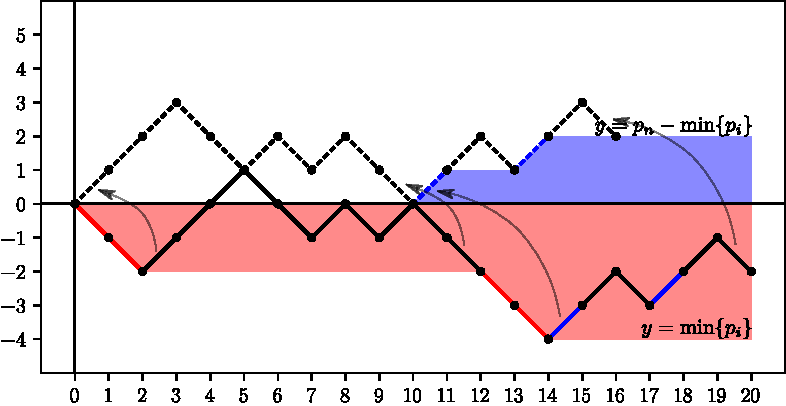
\includegraphics[width = \linewidth]{./img/exchange-arg/bracket-sequence.pdf}
  \caption{\texttt{))((())()())))(()(()} এর জন্য গ্রাফ। প্রথম ধাপে লাল ক্যারেক্টারগুলো ডিলিট হবে। এর পর আমরা লাল অংশগুলো বাদ দিয়ে বাকি অংশগুলোতে একটার পর আরেকটা জোড়া দিলে ডোরাকাটা গ্রাফটি পাবো। সেই গ্রাফের নীল ক্যারেক্টারগুলো ডিলিট করা হবে দ্বিতীয় ধাপে। মোট লাল আর নীল ছায়া করা অংশ দুটি  ডিলিট হবে, যা হলো $p_n - 2\min\{p_i\}$।}
\end{figure}
খেয়াল করো, কিছু স্ট্রিং রিঅ্যারেঞ্জ করে জোড়া লাগানোর পর সেই বড় স্ট্রিং এর $p_n$ আর $\min\{p_i\}$ এর মান আমরা কিন্তু শুধু ছোট স্ট্রিং গুলোর $p_n$ এবং $\min\{p_i\}$ এর মান দেখেই বলে দিতে পারি। আবার ছোট স্ট্রিং গুলো যেভাবেই সাজাও না কেনো বড় স্ট্রিং এর $p_n$ এর মান কিন্তু একই থাকবে (সবগুলো $p_n$ এর যোগফল)। তাহলে আমাদের উত্তর শুধু বড় স্ট্রিং এর $\min\{p_i\}$ এর মানের উপর নির্ভর করছে আর আমাদের উদ্দেশ্য হলো এর মান যতটা সম্ভব বড় করা।

আগের মতই আমরা যেকোনো একটি অপ্টিমাল সলিউশন $O$ নিয়ে ঘাঁটাঘাঁটি করবো। $O$ এর $i$-তম ছোট স্ট্রিংটার $p_n$ কে আমরা $s_i$ আর $\min\{p_i\}$\footnote{এখানে $i$-তম স্ট্রিং এর জন্য খালি $p_i$ বিবেচনা করছি- এরকম না। আসলে সব জায়গায় $\min\{p_i\}$ দিয়ে ঐ স্ট্রিং এর প্রিফিক্স সাম গুলোর মিনিমাম ভ্যালু বুঝানো হচ্ছে।} কে $m_i$ দিয়ে সূচিত করবো। ধরো সব অপ্টিমাল সলিউশনের $\min\{p_i\}$ এর মান $M$ আর যেসব সলিউশনের $\min\{p_i\} \ge M$ তাদের আমরা ভ্যালিড সলিউশন বলবো। তাহলে $O$ যদি একটি অপ্টিমাল সলিউশন হয় তাহলে সব $i$ এর জন্য নিচের শর্তটি পূরণ হবেঃ
\begin{align}
  S + m_i &\ge M \text{ এবং} \label{delMinBra:1}\\
  S + s_i + m_{i+1} &\ge M \label{delMinBra:2}
\end{align}
, যেখানে $S = \sum_{j=1}^{i-1} s_j$। এখন, আমরা যদি $i$ আর $i+1$ সোয়াপ করতে না পারি তাহলে-
\begin{align}
  S + m_{i+1} < M \text{ অথবা} \label{delMinBra:3} \\
  S + s_{i+1} + m_i < M \label{delMinBra:4}
\end{align}
আগের প্রবলেমের মতো এখানে \eqref{delMinBra:2} থেকে কিন্তু আমরা বলতে পারি না \eqref{delMinBra:3} মিথ্যা, কারণ $s_i$ ধনাত্মক, ঋণাত্মক বা শুন্য যেকোনোটিই হতে পারে। তাহলে কি করা যায়? দুটি কেইস আলাদাভাবে চিন্তা করতে পারি আমরা- $s_i$ ধনাত্মক হলে  অবশ্যই সেটাকে একটি  ঋণাত্মক বা শুন্য $s_{i+1}$ এর আগে রাখা উচিত, কারণ আগে রাখলে আমাদের কোনো লস হচ্ছে না বরং পরের কোনো স্ট্রিং-এ এই লাভটা কাজে লেগে যেতে পারে। এটাকে আরেক্টু গুছিয়ে বললে হয়- যদি একটি অপ্টিমাল সলিউশনের $s_i \le 0$ এবং $s_{i+1} > 0$ হয় তাহলে আমরা এই দুটি উপাদান এক্সচেঞ্জ করলে যে সলিউশন পাবো সেটিও একটি ভ্যালিড সলিউশন হবে\footnote{প্রমাণ করে দেখো।}। এবার প্রশ্ন হলো $s_i$ আর $s_{i+1}$ দুটোই ধনাত্মক হলে কি হবে? চিন্তা করে দেখো, যদি অপ্টিমাল সলিউশনে $m_i < m_{i+1}$ হয় তাহলে এখানেও এদের সোয়াপ করলে সলিউশনটি ভ্যালিড থাকবে। কিন্তু আমরা এখানে কোনো কারণ ছাড়া এক্সচেঞ্জ করছি কেন মনে হতে পারে। আগের এক্সচেঞ্জ এর উদ্দেশ্য ছিল সলিউশন ভ্যালিড রেখে আমাদের কিছু প্রফিট আদায় করা, যেগুলো আমরা পরে খরচ করতে পারবো। এখানেও একই। আমরা যদি $m_i > m_{i+1}$ অর্ডারে রাখি তাহলে পরে বৃহত্তর লস ($m$ ভ্যালু গুলোকে লস মনে করো) এর জন্য আমরা আগে থেকে বাঁচিয়ে রাখা কিছু প্রফিট $(s_i)$ ব্যবহার করতে পারবো।\\
এবার আসা যাক $s_i$ আর $s_{i+1}$ উভয়ই ঋণাত্মক বা শুন্য হলে কি হবে। খেয়াল করো, এখন কিন্তু আমরা \eqref{delMinBra:2} থেকে বলতে পারি \eqref{delMinBra:3} মিথ্যা! এখন \ref{pillow_tower} প্রবলেম এর মতো করে আমরা এরকম একটা অসমতা পাবোঃ
\begin{equation}
  s_i - m_i > s_{i+1} - m_{i+1} \label{delMinBra:5}
\end{equation}
তাহলে শেষ পর্যন্ত এই দাঁড়ালো- প্রথমে সব ধনাত্মক $s_i$ কে আগে রাখতে হবে আর বাকি গুলো পরে। তারপর ধনাত্মক $s_i$ গুলোর মধ্যে আমরা $i < j$ এর জন্য $m_i > m_j$ অর্ডারে সাজাবো আর ধনাত্মক বা শুন্য $s_i$ গুলোর ক্ষেত্রে আমরা $i < j$ এর জন্য $s_i - m_i > s_j - m_j$ অনুযায়ী সাজাবো। এই Comparator টা কিন্তু একটা Complete Order\footnote{ভেরিফাই করে দেখো।}!\\
এখন কিন্তু আরেকটি কাজ বাকি রয়ে গিয়েছে! আমরা ধরে নিয়েছিলাম আমরা সোয়াপ করতে পারবো না অর্থাৎ সোয়াপ করলে সলিউশনটা ইনভ্যালিড হয়ে যাবে। কিন্তু সোয়াপ করলে পারলে \eqref{delMinBra:5} অনুযায়ী সাজালেও যে সেটি একটি ভ্যালিড সলিউশন থাকবে তা প্রমাণ করতে হবে। এটা \ref{pillow_tower} প্রবলেমটির মতো করে প্রভ করার চেষ্টা করো।
\end{solution}

\section{অনুশীলনী}

\begin{exercise}[\href{https://codeforces.com/problemset/example/1354/F}{Codeforces 1354F - Summoning Minions}]
তোমার কাছে $n \, (1 \le n \le 75)$-টা মিনিয়ন আছে এবং তুমি তাদের হাজির করতে পারো। $i$-তম মিনিয়নের প্রথমিক পাওয়ার লেভেল হলো $a_i \, (1 \le a_i \le 10^5)$, এবং যখন তুমি এই মিনিয়নটিনে হাজির করবে, তখন আগের মিনিয়ন সবগুলোর পাওয়ার $b_i \, (0 \le b_i \le 10^5)$ করে বেড়ে যাবে। মিনিয়নগুলোকে তুমি যেকোনো ক্রমে হাজির করতে পারবা। কিন্তু একটা শর্ত আছে, তুমি যেকোনো সময় $k \, (1 \le k \le n)$ টার বেশি মিনিয়ন হাজির করে রাখতে পারবে না। তুমি যেকোনো সময় হাজির করা মিনিয়নকে ধ্বংস করে দিতে পারবা -- অন্যভাবে বলতে গেলে, প্রতিটা মিনিয়নকে তুমি সর্বোচ্চ একবার হাজির (বা ধ্বংস) করতে পারবা। তোমার লক্ষ্য হলো সবচাইতে শক্তিশালী মিনিয়নের আর্মি হাজির করা, অর্থাৎ, শেষ পর্যন্ত থাকা (যেগুলো হাজির করেছ, কিন্তু ধ্বংস করোনি) মিনিয়নগুলোর পাওয়ার লেভেলের যোগফল ম্যাক্সিমাইজ করা। প্রতিটা ইনপুট ফাইলে $T \le 75$ টা টেস্ট কেইস থাকতে পারে।
\end{exercise}
